% !TeX root = creno_tr.tex
%=======================================================================================
\section{Introduction}\label{Introduction}

The first IETF RFC to define the CUBIC congestion control algorithm~\cite{Rhee18:Cubic_RFC} was based on the original paper introducing CUBIC~\cite{Ha08:cubic}. For `TCP-friendly' mode, both draw on an equation in an ACIRI technical report~\cite{Floyd00:Eqn_v_AIMD_cc} when they specify the additive increase factor. The derivation of the equation in that technical report assumes a deterministic dropping (or ECN-marking) algorithm at the bottleneck, which limits its applicability. Also the technical report attempts to validate the theoretical formula empirically by simulation using a RED gateway at the bottleneck, but it leads to flow rates that are significantly different (by a factor of more than 2\(\times\)) when they should be the same.

Below, an equation for the additive increase factor is derived without the assumption of deterministic dropping. Instead it is assumed that drops are synchronized between flows, which is typically the case for tail-drop queues. The resulting equation turns out to be the same as that in the technical report~\cite{Floyd00:Eqn_v_AIMD_cc}. However, the derivation here is a straightforward geometric one. It relies on fewer assumptions and no approximations; it considers variation of the RTT explicitly and it does not use loss probability at all.

The present paper is not intended to be ambitious or insightful, just pedestrian and rigorous. \cite{Bansal01:Binom_cc} provides and analyses a wider set of TCP-friendly algorithms, but does not dwell on the simple linear cases analysed here.

\section{Terminology}\label{Terminology}

Nowadays, TCP-friendly mode is more accurately known as Reno-friendly mode, given its flow rate is intended to match that of the Reno congestion control, and given that it is irrelevant which wire protocol is used, whether TCP, QUIC, SCTP, etc. The term C-Reno will be used for CUBIC in Reno-friendly mode.

This paper uses the variables defined below:
\begin{description}[nosep]
	\item[\(a\)]: Additive increase factor;
	\item[\(b\)]: Multiplicative decrease factor;
	\item[\(j\)]: Round index;
	\item[\(J\)]: Rounds per sawtooth cycle;
	\item[\(R(j)\)]: Round trip time (RTT);
	\item[\(W(j)\)]: Congestion window;
	\item[\(\widehat{W}\)]: Maximum \(W\);
	\item[\(r(j)\)]: Packet rate;
	\item[\(X_r\)]: Reno variant of any variable \(X\);
	\item[\(X_c\)]: C-Reno variant of any variable \(X\).
\end{description}

\section{AIMD-Friendliness}\label{AIMD-Friendliness}

Consider two types of Additive Increase Multiplicative Decrease (AIMD) flow with parameters (\(a_r, b_r\)) and (\(a_c, b_c\)) competing at a bottleneck, under the following assumptions:
\begin{itemize}[nosep]
	\item The buffer is large enough not to drain completely, even if all flows reduce simultaneously (this assumption is relaxed later).
	
	\item All other factors of all the flows, particularly packet size and base RTT, are equal. When flows sharing the same bottleneck queue all have the same base RTT, they all have the same RTT, \(R(j)\),  at every stage, \(j\), of their sawtooth cycles. 	
	
	\item The bandwidth-delay product (BDP) is low enough for all flows to remain in their AIMD mode throughout the cycle.

	\item All the flows have run long enough to converge to a steady state.

	\item All flows only respond to the presence of loss, not its extent.
\end{itemize}

\begin{figure*}
	\centering
	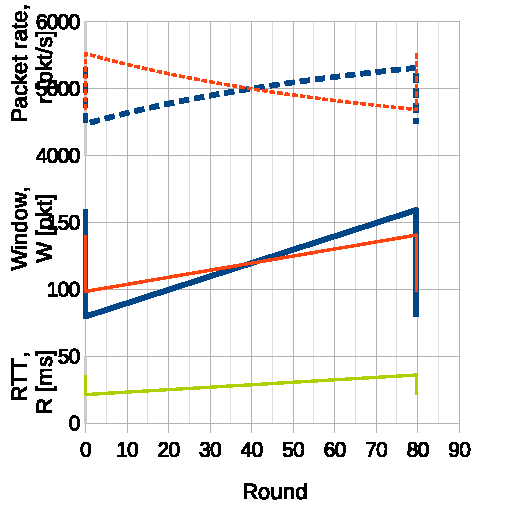
\includegraphics[height=6.5cm]{creno-synch-round}
	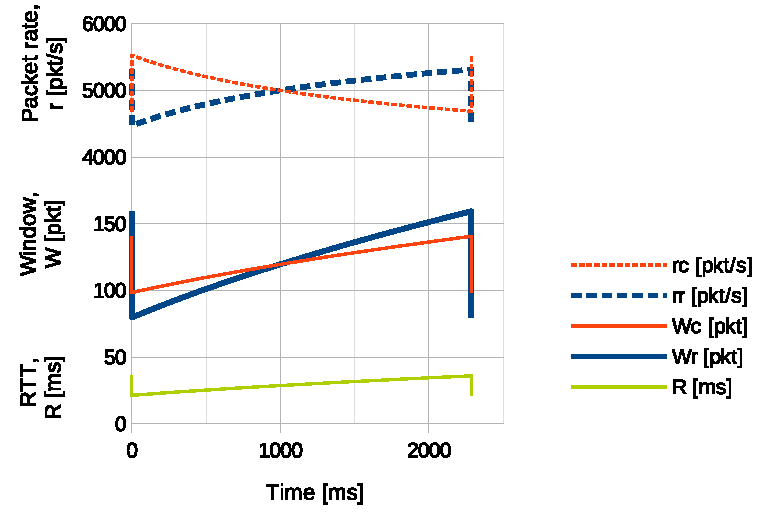
\includegraphics[height=6.5cm]{creno-synch-time}
	\caption{One synchronized sawtooth cycle of C-Reno and Reno plotted wrt.\ round trips (left) and wrt.\ time (right)}\label{fig:creno-synch}
\end{figure*}

% ----------------------------------------------------------------
\subsection{Synchronized (Tail-Drop) Case}\label{Synch}

For this case, it is additionally assumed that:
\begin{itemize}[nosep]
	\item All the flows are synchronized so that, whenever one flow experiences loss the others do too;

	\item All flows experience at least one loss at each congestion event (relaxation of this assumption is discussed later);
\end{itemize}

\paragraph{Steady state:} For each flow, the additive increase of a cycle balances with its multiplicative decrease from the max, \(\check{W}/b\), to the min, \(\check{W}\). 
\begin{align}
	a_r J &= \widehat{W}_r - b_r\widehat{W}_r\notag\\
	      &= \widehat{W}_r(1-b_r)\label{eqn:ssr}\\
	a_c J &= \widehat{W}_c(1-b_c)\label{eqn:ssc}
\end{align}

\paragraph{Flow rate equality:} Given the parameters \(a_r, b_r, b_c\) the aim is to derive \(a_c\) such that each flow's average rate is the same. This is equivalent to each flow transferring the same number of packets over a cycle. 

As a cycle progresses, the RTT grows. So to derive the number of packets transferred over a cycle, the packet rate has to be weighted by the RTT in each cycle before being summed:
\begin{align}
	\sum_{j=0}^{J-1} r_c(j) R(j) &= \sum_{j=0}^{J-1} r_r(j) R(j)\notag\\
	\sum_{j=0}^{J-1} W_c(j) &= \sum_{j=0}^{J-1} W_r(j)\label{eqn:cwnd_equality}\\
	\sum_{j=0}^{J-1} b_c\widehat{W}_c + a_c j &= \sum_{j=0}^{J-1} b_r\widehat{W}_r + a_r j\notag\\
	Jb_c\widehat{W}_c +\frac{J^2 a_c}{2} &= Jb_r\widehat{W}_r +\frac{J^2 a_r}{2}\notag\\
\intertext{Dividing through by \(J\) and substituting from \autoref{eqn:ssr} \& \autoref{eqn:ssc}:}
    \widehat{W}_c \left(b_c + \frac{(1-b_c)}{2}\right) &= \widehat{W}_r \left(b_r + \frac{(1-b_r)}{2}\right)\notag\\
	\frac{\widehat{W}_c}{\widehat{W}_r} &= \frac{(1+b_r)}{(1+b_c)}\label{eqn:fre}
\end{align}
Returning to the steady state equations, we can divide \autoref{eqn:ssc} by \autoref{eqn:ssr}, then substitute from \autoref{eqn:fre}:
\begin{align}
	\frac{a_c}{a_r} &= 
	                 \frac{\widehat{W}_c}{\widehat{W}_r}\frac{(1-b_c)}{(1-b_r)}\notag\\
	                &= \frac{(1-b_c)}{(1+b_c)}\frac{(1+b_r)}{(1-b_r)}\label{eqn:friendly}
\end{align}
Plugging in Reno's AIMD factors, \(a_r=1, b_r=1/2\):
\begin{equation}
                \boxed{a_c = \frac{3(1-b_c)}{(1+b_c)}}\label{eqn:reno-friendly}
\end{equation}
\begin{figure*}
	\centering
	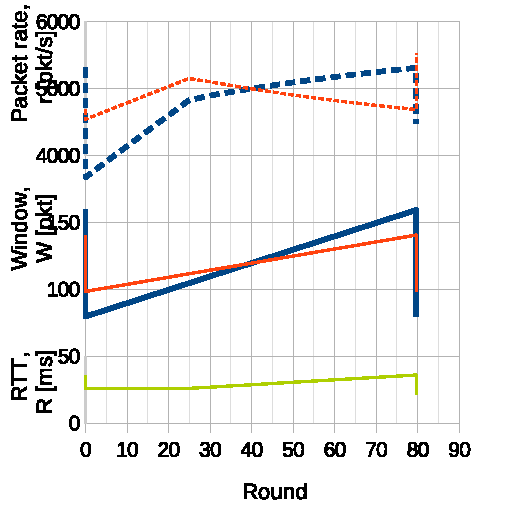
\includegraphics[height=6.5cm]{creno-synch-round-shallow}
	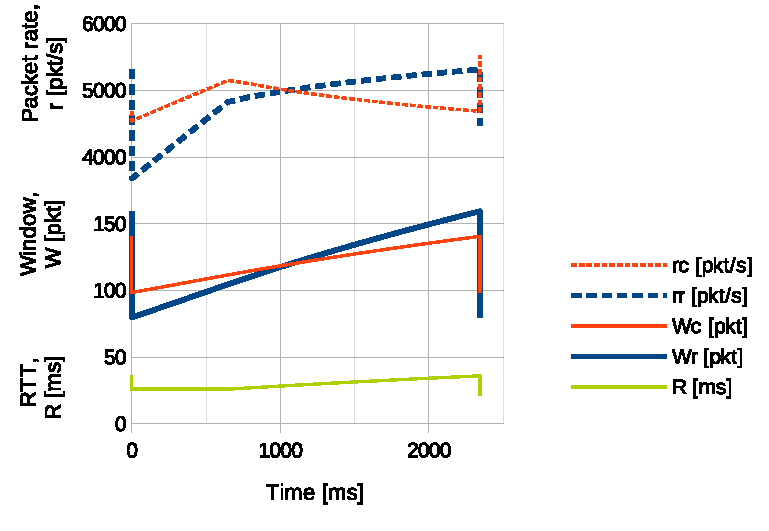
\includegraphics[height=6.5cm]{creno-synch-time-shallow}
	\caption{Similar synchronized sawtooth cycle of C-Reno and Reno to \autoref{fig:creno-synch}, but with a 11\,ms buffer that is too shallow to accommodate both sawteeth at once.}\label{fig:creno-synch-shallow}
\end{figure*}And plugging in the multiplicative decrease factor of C-Reno recommended in \cite{Rhee18:Cubic_RFC}, \(b_c=0.7\):
\begin{align*}
               a_c  &= 9/17\\
                    &\approx 0.53.
\end{align*}

\paragraph{Geometric interpretation:} \autoref{fig:creno-synch} shows one flow each of C-Reno and Reno competing over one synchronized sawtooth cycle. Superficially, the whole derivation of \(a_c\) above can be derived from simple triangle geometry, by drawing congestion window sawteeth that increase linearly wrt.\ round trips (mid-left) then setting the mid-points of the two ramps to the same height. Then \autoref{eqn:fre} gives the ratio between the heights of the bases of the triangles, and \autoref{eqn:friendly} gives the ratio of the heights of the triangles themselves.

However, it is not enough to merely assert that the average heights of these sawteeth are equal, as \cite{Floyd00:Eqn_v_AIMD_cc} does. Strictly, it is necessary to start from the goal of equal flow rates averaged over time, as the above analysis does. Given RTT grows throughout the cycle, the plots of flow-rate against time (top right in \autoref{fig:creno-synch}) stretch out more to the right, forming concave curves. It is not at all obvious how to equate the averages of these two curves until they are weighted by round trip duration, which transforms them into the linear plots of window wrt.\ rounds (mid-left), as in \autoref{eqn:cwnd_equality}.

It is also interesting to note from \autoref{fig:creno-synch} that C-Reno's packet rate \emph{decreases} as its window increases over the sawtooth. This is because the competing Reno flow causes the RTT to grow faster than would be the case with only C-Reno flows. 

If the buffer is not deep enough to hold all the synchronized sawteeth, it will be empty during the early part of the sawteeth. Then both flows will under-perform during the early part of the cycle when C-Reno would have achieved its highest packet rate and Reno would have achieved its lowest, as shown in \autoref{fig:creno-synch-shallow}. Nonetheless, the rate of both flows reduces proportionately, so the ratio between their flow rates remains unaltered.

\paragraph{Synchronized losses?} We will now question the assumption that each flow always catches at least one loss at each congestion event. We still consider two flows with equal RTTs: 1 Reno and 1 CReno. Between responses to losses, the queue grows inexorably by \((a_r + a_c \approx 1.53)\) pkt/RTT. Every time the buffer fills, one packet has to be dropped, but the queue continues to grow by 1.53 segments during the next round trip (until the resulting response reaches the queue). So it is likely that another packet will have to be discarded within the same RTT as the first.

The likelihood that a particular flow catches any one of the losses depends on its packet rate relative to the other.\footnote{Irrespective of how rapidly the flow's own window is growing.}
If the flows both have the same average window (our goal, as shown in \autoref{fig:creno-synch})
then, by \autoref{eqn:fre} (or triangle geometry), the ratio between the packet rates of the two flows when they both reach their max is
\begin{figure*}
	\centering
	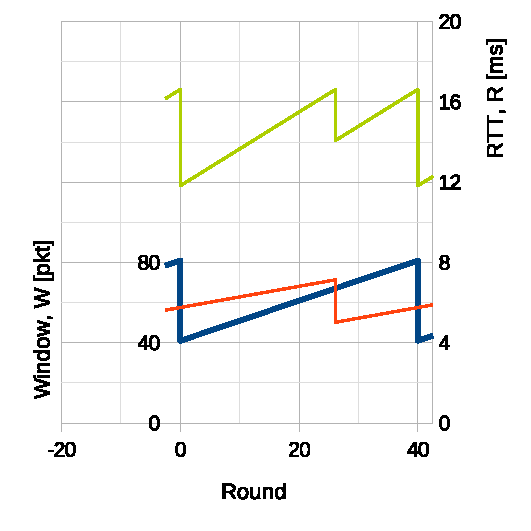
\includegraphics[height=6.4cm]{creno-determ-round}
	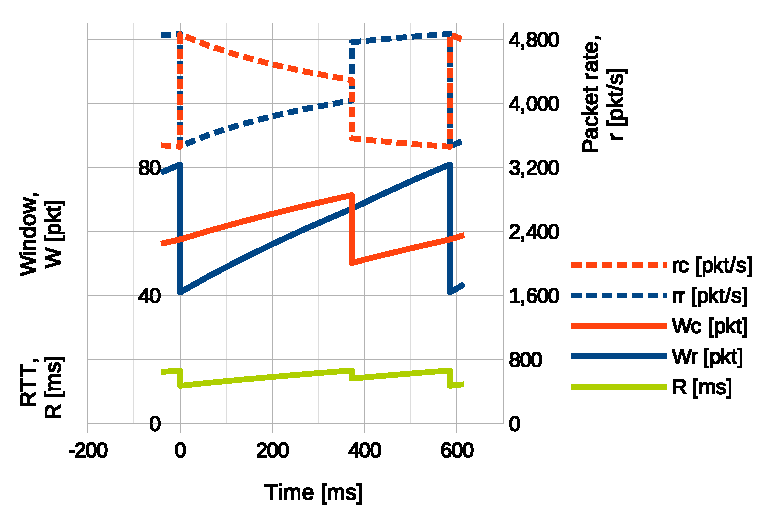
\includegraphics[height=6.4cm]{creno-determ-time}
	\caption{One desynchronized sawtooth cycle of C-Reno and Reno plotted wrt.\ round trips (left) and wrt.\ time (right)}\label{fig:creno-determ}
\end{figure*}

\begin{align}
\frac{\widehat{r_r}}{\widehat{r_c}} &= \frac{(1 + b_c)}{(1 + b_r)}\notag\\
        &= \frac{1.7}{1.5}\notag\\
        &\approx 1.13.\label{eqn:r_ratio}
\end{align}

When a loss occurs, from \autoref{eqn:r_ratio}, we can say that:
\begin{align}
p_r / p_c = 17/15\label{eqn:p_ratio}\\
p_r + p_c = 1.
\end{align}
Therefore
\begin{align*}
p_r &= 17/32 &\approx 53\%\\
p_c &= 15/32 &\approx 47\%
\end{align*}
Then, for example, if there are two losses during a congestion event, the probabilities of each combination of two losses are:
\begin{align*}
p_{rr}              &= (17/32)^2               &&\approx 28\%\\
p_{rc} \lor p_{cr}  &= 17*15/32^2 + 15*17/32^2 &&\approx 50\%\\
p_{cc}              &= (15/32)^2               &&\approx 22\%,
\end{align*}
where \(p_{ij}\) is the probability of a loss from flow \(i\) then \(j\).

When there are two losses in a round and the same flow is hit twice, it doesn't reduce any more than if it's hit once, but the other flow doesn't reduce at all. So CReno is somewhat more likely than Reno to not get hit in some round. In such cases, only the Reno flow would reduce, then the queue would continue to grow by \((a_r + a_c \approx 1.53)\) pkt/RTT, so the next cycle would be shorter and the CReno flow would be much more likely to be hit when it next filled the buffer --- and more likely to be hit twice.

It would be possible to calculate the average rate of each type of flow by calculating the probabilities of each chain of events programmatically. However, such precision is unnecessary. For the case of tail-drop buffers, it will be sufficient to say:
\begin{itemize}
	\item either that the AI factor of CReno should be slightly lower than that derived from \autoref{eqn:reno-friendly} to make CReno and Reno flow rates more precisely equal;
	\item or that the average rate of CReno flows will be slightly higher in comparison with Reno flows, if \autoref{eqn:reno-friendly} is used.
\end{itemize}
Here, `slightly''  means roughly within a 10\% margin of error.

% ----------------------------------------------------------------
\subsection{Desynchronized (AQM) Case}\label{AQM}

For this case, instead of the assumption of synchronization, it is assumed that:
\begin{itemize}[nosep]
	\item As the queue grows, Active Queue Management (AQM) at the bottleneck selects single packets to drop or mark, so that the congestion responses of each flow tend not to coincide.\footnote{In desynchronized cases, the RTT varies less than in synchronized cases---on average the amplitude is respectively \(1/\sqrt{n}\) vs.\ \(n\) times that of a single flow, where \(n\) is the number of flows~\cite{Appenzeller04:Sizing_buffers}. Therefore, the first assumption listed in \S\,\ref{AIMD-Friendliness} (that the buffer is large enough not to drain completely) is much more likely to hold in desynchronized cases.}
\end{itemize}

The AQM case is harder to analyse than the synchronized case with tail-drop. Superficially, one could use the transformation from equal average flow rates (wrt.\ time) into equal window (wrt.\ rounds). However, there is no guarantee that the number of rounds per cycle, \(J\) is the same in each case.

If we assumed it was, we would end up with \autoref{eqn:reno-friendly} for C-Reno's additive increase factor \(a_c\). Then, as shown in \autoref{fig:creno-determ}, the phasing between the sawteeth would evolve so that the queue reached roughly the same depth before each reduction, i.e.\ the tips of the RTT sawteeth will all align at roughly the same level---the operating point of the AQM. 

However, although \autoref{fig:creno-determ} shows the sawtooth reductions alternating Reno -- C-Reno -- Reno, this need not be the case. In the cycle after 400\,ms in the top-right plot, the ratio between C-Reno's and Reno's packet rates is about 51:49. So it is nearly as likely that the AQM will hit a Reno packet as a C-Reno packet, causing Reno to reduce twice in a row. If the AQM did hit C-Reno around 400\,ms, at around 600\,ms the ratio would be about 42:58, making Reno more likely to be hit. Overall, if \(a_c\) is set as for the synchronized case (\autoref{eqn:reno-friendly}), an AQM is likely to hit Reno somewhat more often than C-Reno.

\begin{figure}
	\centering
	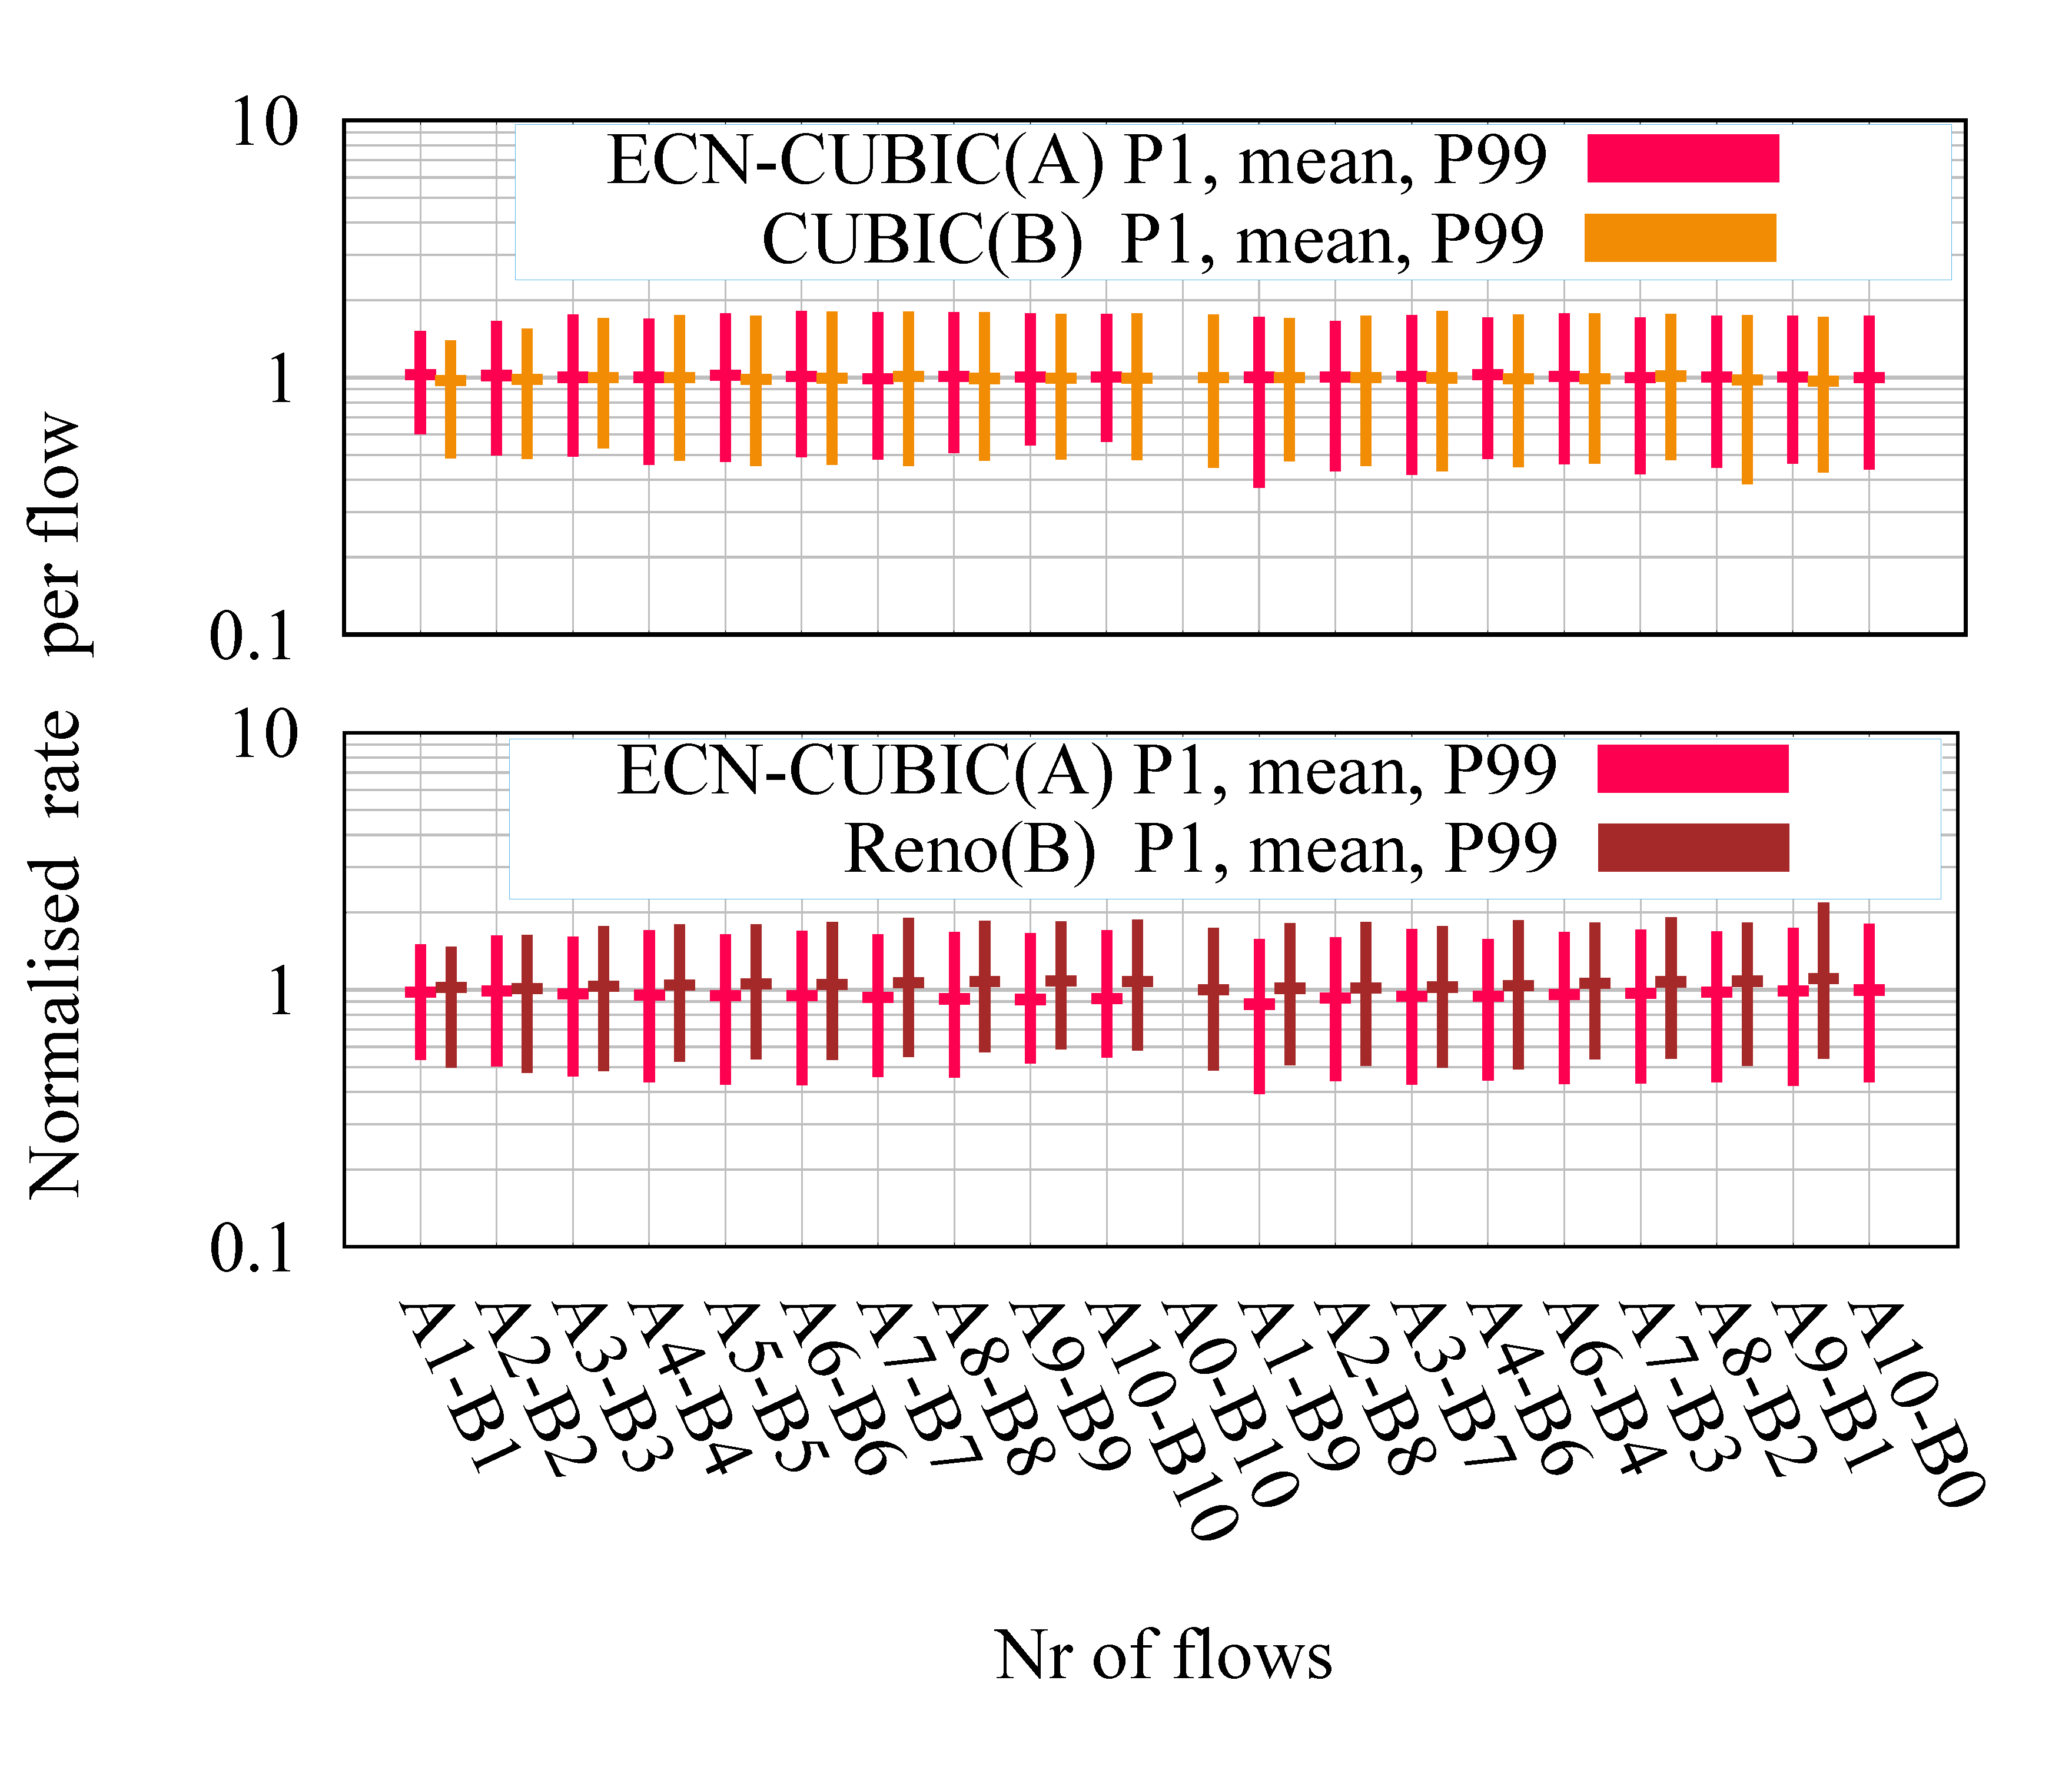
\includegraphics[width=\linewidth]{ts_link40_rtt10_reno-PIE}
	\caption{AQM: PIE; link capacity: 40\,Mb/s; Base RTT: 10\,ms.}\label{fig:creno-v-reno-PIE}
\end{figure}
\paragraph{Empirical Results:} Lon-running CReno flows with \(b_c = 0.7\) and AI factor \(a_c=1.53\) were tested against Reno over a path with base RTT 10\,ms containing a PIE AQM at the 40\,Mb/s bottleneck. Various combinations of numbers of each flow type were used, as shown along the \(x\)-axis of \autoref{fig:creno-v-reno-PIE}. For instance, in the top plot, A2-B8 means 2 ECN-CUBIC flows vs. 8 (non-ECN) CUBIC flows. And in the bottom plot it means 2 ECN-CUBIC flows vs. 8 (non-ECN) Reno flows.\footnote{In each run flow rate measurement was delayed until the flows had converged, then taken every second for 250\,s. The resulting 250 measurements were analysed to calculate the percentiles. The two types of flow were sent from two sendering hosts to two receiving hosts via a bridge and a bottleneck AQM node. All machines were running Linux kernel v5.10.31. All CCs and AQMs were configured with default parameters.}

The whisker plots show 1\textsuperscript{st} \%-ile (P1), mean and 99\textsuperscript{th} \%-ile (P99) normalized flow rate. Normalized flow rate is defined as the flow rate relative to \(\sfrac{1}{N}\) of the capacity, where \(N\) is the total number of flows.

It can be seen that CReno seems to be slightly less aggressive than Reno under these conditions. However, the discrepancy is hardly visible, and more than an order of magnitude smaller than the range of the ratio's natural variability between its P1 and P99.

In the simulations using the RED AQM in Floyd's report~\cite{Floyd00:Eqn_v_AIMD_cc}, CReno throughput was 70\% of that of competing Reno flows when C-Reno used \(b_c=7/8\) and \(a_c\) was set according to  \autoref{eqn:reno-friendly}. No-one has been able to explain those results. However, the present report shows that \autoref{eqn:reno-friendly} is at least sufficient for the Reno-Friendly algorithm in CUBIC with the widely deployed decrease factor of \(b_c=0.7\).

